\section{Revisão Bibliográfica} \label{chap:revisao_bibliografica}

\subsection{FPGAs e Sintetizadores em Alto Nível}

%Neste capítulo será descrito os principais conceitos necessários para o entendimento base dos fundamentos do trabalho, além de suas tecnologias e metodologias.

%\subsection{\textit{Field-Programmable Logic Device} (FPGA)}

	% uso de fpga no mundo
	Até recentemente, os \hardwares\ reconfiguráveis eram utilizados unicamente na prototipação de projetos de circuitos integrados de aplicação especifica (ASIC) e produção em baixo volume por causa de sua baixa velocidade e custo por unidade.
	Mas com a variedade desses dispositivos disponibilizados hoje no mercado, em conjunto com a elevação do custo de engenharia não recorrente, houve um crescente interesse na utilização de FPGAs para sistemas embutidos devido suas vantagens sobre ASICs em termos de flexibilidade de projeto e custo zero de engenharia não recorrente \cite{Mei2000}. 
	%lousa branca
    \begin{comment}
	Tais dispositivos, juntos com sua plataforma de interação, de forma geral, permitem ao \designer\ de sistemas embutidos ter uma \textit{lousa branca} em que possa implementar \hardwares\ computacionais personalizados tão facilmente como o desenvolvimento de um \software, como foi possível ilustrar na Figura \ref{fig:rt-board}.
	% Plataforma FPGA
	Dessa forma, uma \textit{plataforma FPGA} é um chip na qual contém o componente FPGA integrado à inúmeras interfaces e componentes desde LEDs (do inglês \textit{Light-Emitting Diode}) e \textit{switchs} até porta Ethernet e interface vídeo VGA (do inglês \textit{Video Graphics Array}) e como possui recursos suficientes para circuitos complexos, é possível implementar funções de processamento de imagem, interfaces de rede, algoritmos criptográficos e processadores completo de acordo com sua capacidade. %\cite{Plessl2003}
	Entretanto, enquanto configurar um \hardware\ reconfigurável é uma tarefa fácil graças às ferramentas disponíveis hoje, criar um \design\ de \hardware\ inicial não é \cite{Sass2010}.

	\begin{figure}[h] \centering
		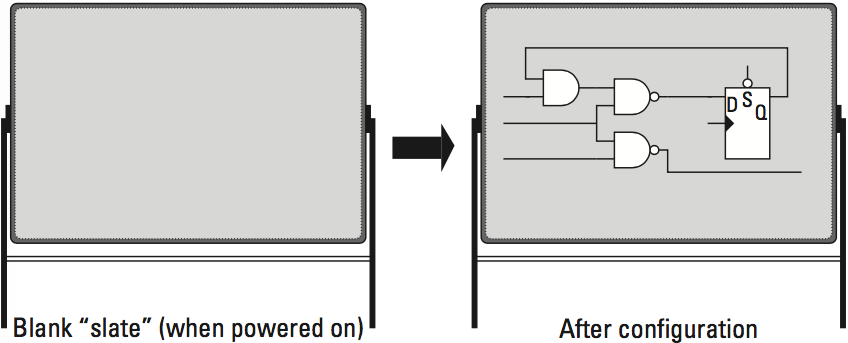
\includegraphics[width=0.75\textwidth]{img/rt-board.png}
		\caption{Ilustração em alto nível do funcionamento interno do FPGA. Fonte: \cite{Sass2010}.}
		\label{fig:rt-board}
	\end{figure}

	A seguir, será descrito a tecnologia que consiste os \hardwares\ reconfiguráveis, em especial o FPGA, e as respectivas linguagens de descrição de \hardware.

	\subsubsection{\textit{Field-Programmable Logic Device} (FPGA)}
		% PLD
		Para introduzir alguns conceitos, é importante destacar o que são os dispositivos lógicos programáveis (PLDs, do inglês \textit{Programable Logic Devices}). Às vezes chamados de dispositivos lógico programáveis em campo (FPLD, do inglês \textit{Field-Programmable Logic Device}), podem ser adaptados para criar muitos dispositivos digitais, desde simples portas lógicas até estruturas complexas. \cite{tocci2003sistemas, Plessl2003} dizem que com um investimento de capital pequeno, qualquer empresa pode comprar os \software\ de desenvolvimento e \hardware\ necessário para programar PLDs para seus projetos digitais. De modo geral, os PLDs são descritos como pertencendo a três tipo diferentes sendo eles os dispositivos lógicos programáveis simples (SPLD), dispositivos lógicos programáveis complexos (CPLDs, do inglês \textit{Complex Programmable Logic Devices}) e arranjo de portas programáveis em campo (FPGA) sendo o último tipo abordado neste trabalho \cite{Brown1996}.

		%LUTS
		Os FPGAs em especial constituem de vários módulos lógicos programáveis relativamente pequenos e independentes interconectados para criar funções maiores. Cada módulo lida, normalmente, com até quatro ou cinco variáveis de entrada. A maioria dos FPGAs utilizam uma \textit{look-up table} (LUT) para criar as funções lógicas desejadas. Uma LUT funciona como uma tabela-verdade, no sentido que a saída é programada para criar a função combinacional armazenando valores verdadeiros e falsos adequado a cada combinação de entrada.
		Os recursos de roteamento de sinal programável dentro do chip tendem a ser bem variados, com extensões de caminhos diferentes disponíveis. Os atrasos de sinal em um projeto dependem do roteamento real de sinal selecionado pelo \software\ de programação. Os módulos lógicos também contêm registradores programáveis. Eles não são associados a nenhum pino de entrada e saída (I/O, do inglês \textit{Input and Output}). Em vez disso, cada pino de I/O é conectado ao bloco programável de entrada e saída que, por sua vez, é conectado aos módulos lógicos com linhas de roteamento selecionadas.
		\todo{figura fpga}
        Os blocos de I/O podem ser configurados para fornecer recursos de entrada, saída ou bidirecionais, e registradores internos, usados para guardar dados que entram ou saem. Uma arquitetura geral de FPGA com 16 blocos lógicos é exibida na Figura \ref{fig:rt-arch_fpga}.
        Todos os blocos lógicos e os de entrada e saída implementam qualquer circuito lógico. As interconexões programáveis são estabelecidas por meio de linhas que passam pelas linhas e colunas nos canais entre esses blocos \cite{tocci2003sistemas}.
	%A tecnologia interna de um FPGA consiste basicamente de um arranjo de blocos lógicos, canais de roteamento para interconexão de blocos lógicos e blocos de entrada e saída de sinais em torno do circuito.
	FPGAs baseado em SRAM (do inglês \textit{Static Random Access Memory}) utilizam células SRAM para controlar a funcionalidade de blocos lógicos e entrada e saída de sinais bem como as rotas, e pode ser reprogramado arbitrariamente em nível de circuito, muitas vezes, baixando um novo \textit{stream} de dados de configuração para o dispositivo.
	Hoje, esses dispositivos possuem milhões de portas de lógica programável, bilhões de transistores, além de outros blocos de \hardware\ dedicados dedicados como rápidas memórias embarcadas e multiplicadores de ponto-fixo tornado-o um dos circuitos integrados (CI) mais densos existente \cite{Choi2016}.
    \end{comment}

		\begin{comment}

		\begin{figure}[h] \centering
			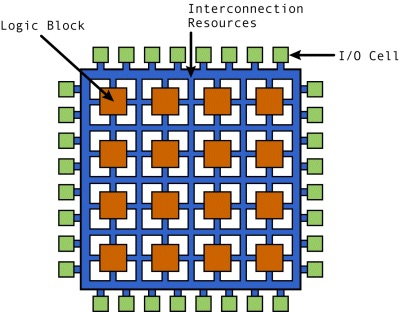
\includegraphics[width=0.5\textwidth]{img/rt-arch_fpga.jpg}
			\caption{Exemplo da arquitetura internas de um FPGA. Fonte: \url{http://www.eetimes.com/document.asp?doc_id=1274496}. Acesso: 30/05/2017.}
			\label{fig:rt-arch_fpga}
		\end{figure}
		\end{comment}


	\begin{comment}
		% tecnologia e energia
		Segundo \cite{tocci2003sistemas}, tais maravilhas de flexibilidade de projetos digital utilizam tecnologia CMOS e podem fornecer uma série de opções de projeto sendo voltados para indústria e até mesmo educação. 
        Ao utilizar tecnologia CMOS, o consumo de energia do chip é relativamente baixo comparado com outras tecnologias podendo ser confeccionado em nível de tensão elétrica, frequências e cargas para os sinais de I/O. O mercado fornece diferentes graus de velocidade de FPGA a fim de que o projetista utilize o mais adequado ao projeto.

		Um dispositivo FPGA pode ser configurado para um número infinito de projetos, de maneira que não é possível simplesmente afirmar o montante de dissipação de energia para um dispositivo FPGA. %O \software\ Quartus II tem duas ferramentas para estimular o montante de uso de energia para uma aplicação. %O \textit{PowerPlay Early Power Estimator} é usado durante os estágios iniciais do projeto para estimar a magnitude de potência do dispositivo.
		Dessa forma, FPGAs são chips que podem ser programados instantaneamente para funções de qualquer circuito digital \cite{Choi2016}.
    \end{comment}

		% Importancia
		Os autores \cite{tocci2003sistemas, Plessl2003} citam que o motivo de PLDs estarem dominando o mercado é o fato de que, como são dispositivos programáveis, a mesma funcionalidade pode ser obtida com um circuito integrado (CI), em vez de com diversos circuitos individuais. 
        Isso significa menor espaço ocupado na placa, menor consumo de energia, maior confiabilidade, menor complexidade de desenvolvimento e, geralmente, menor custo de fabricação.

		%Um das maiores barreiras para o \design\ de projetos em FPGA é a necessidade de uso de linguagem de Descrição de \Hardware\ (do inglês \textit{Hardware Description Language}). HDL é uma das classes de linguagens de computação usados para descrever formalmente um circuito eletrônico. Uma expressão padrão baseada em texto HDL é capaz de descrever o comportamento temporal ou a estrutura de circuito (espacial) de um sistema eletrônico. Sua origem veio da raiz da necessidade de documentar o comportamento do \hardware \cite{Sass2010}.

		%HDL é amplamente utilizado em \design\ de \hardware\ especificando detalhes de \design\ de chip para tantos chips específicos quantos os próprios FPGAs. Para customizar algum tipo de algum chip lógico digital específico, HDLs especifica um modelo para um comportamento específico de um circuito antes do circuito ser projetado e construído. Ferramentas lógicas de sínteses são invocadas em seguida para gerar informações geométricas que são utilizadas para produzir as máscaras \textit{photolithographic}, necessárias para a fabricação do CI do projeto desenvolvido.

		%A utilização de uma HDL é o primeiro passo no processo de síntese. O código é entregue ao compilador lógico, chamado de ferramenta de síntese, e sua saída será carregada ao dispositivo reconfigurável.
		%A propriedade única deste processo e que fornece a lógica programável em geral é que, com esse processo, é possível alterar o código HDL muitas vezes, compilá-lo e fazer seu \textit{upload} no mesmo dispositivo para testar quantas vezes forem necessárias sem custo adicional \cite{Smith1998}.

		Enquanto a maioria de engenheiros de \hardware\ utilizam tanto o \textit{VHDL} quanto o \textit{Verilog}, na qual possuem um nível elevado de complexidade \cite{Choi2016}, existe outras linguagens disponíveis para uso como \textit{SystemC}, \textit{HandelC} e \textit{Impulse}. Fornecem a construção de sistemas \hs\ juntos, dando ao \designer\ uma linguagem de alto nível para manuseio do projeto \cite{Sass2010}.


	%\subsection{\textit{High-Level Synthesis} (HLS)}
		Sintetizadores em Alto Nível (HLS, do inglês \textit{High-Level Synthesis}) são procedimentos que sintetizam códigos em alto nível para HDLs. Realizado uma especificação de \design\ em \software, um HLS pode reduzir os longos ciclos do processo de \design\ de \hardware\ e ainda trazer melhoria em performance e eficiência energética \cite{Choi2016}.

		As primeiras ferramentas sistetizadores baseavam em linguagem \textit{C} mas não houve um sucesso em seu uso pois os engenheiros de \hardware\ acreditam que existe uma lacuna entre o HLS e o \design\ de \hardware\ feito por humanos por parte das ferramentas HLS não explorarem profundamente o recurso de paralelismo, além de que, para os engenheiros de \software\ HLS continua sendo uma dificuldade já que muitas partes do projeto, como a integração do sistema, permanecem em grande parte como um processo manual. Ferramentas como o \textit{framework} LegUp possuem o propósito de entregar um bom HLS além de tentar amenizar esses problemas de projetos \cite{Canis2013}.

		Para prover um melhor suporte para o paralelismo em \hardware, utilizaram de bibliotecas \textit{multi-threads} como a \textit{Pthread} \cite{Barney2009}, \textit{OpenMP} \cite{openmp}, OpenCL \cite{Trevett2008} para criar aceleradores em \hardwares\ paralelos. É investigado otimizações em memória e arquitetura de sistema provendo melhorias em performance de circuito, área, utilizando uma abordagem do padrão produtor-consumidor para inferir circuito de transmissão em \hardware.

\begin{comment} %comment Módulos e Interfaces em \Design\ de \Software
\subsection{Conceitos e Componentes de \Design\ de Sistemas}
	% \subsubsection{Módulos e Interfaces}
	%Existem duas filosofias de \design\ para a construção de um sistema. Em um delas é possível realizar a especificação de cada função do projeto, chamado de blocos básicos\footnote{Um bloco básico é uma sequência maximal de instruções sequenciais com \textit{single entry and single exit} (SESE).}, e conectá-los logicamente de acordo a fim gerar o sistema completo. Tal é descrito como abordagem \textit{bottom-up}.
	%A segunda baseia-se na descrição de um sistema completo e geral sendo que, em seguida, o \designer\ desmembra-o definindo seus sub-blocos até chegar ao nível mais básico de suas funções. Essa é chamada de abordagem \textit{top-down}.
	%O conceito de abordagem de desenvolvimento de projetos é importante para descrever os conceitos de módulo e interface.%, segundo \cite{Sass2010}.



	\subsubsection{Módulos e Interfaces em \Design\ de \Software}
		\cite{Sass2010}, em seu livro, descreve que módulo é qualquer conjunto de operação auto-contidas que possui um nome, interface formal e geral e alguma descrição funcional. Isso significa que qualquer procedimento, mesmo que em \software\ ou em descrição de \hardware, que possa ser representado por uma caixa graficamente é considerado um módulo.
		Define-se por interface formal o nome do módulo e a enumeração de duas operações, incluindo suas entradas e saídas, caso existam e a interface geral inclui todas as características da interface formal e qualquer protocolo ou comunicação adicional implícita. Com a interface formal descrita, é possível realizar inspeções mecânica e técnica no módulo enquanto a geral, o entendimento desse em alto nível.
		Por último, um módulo pode ter também uma descrição funcional no qual pode ser implícita, formal ou informal. Quando a descrição é implícita, a descrição está presente de forma clara no nome do módulo, como por exemplo \texttt{full\_adder}. A formal consiste na documentação ou em meios matemáticos e comentários formais sobre as operações do módulo e a informal pode ser comentários descritivos ao longo da escrita da função.

		Outros termos importantes são implementação e instância. Uma implementação é a realização de uma funcionalidade pretendida de um módulo mesmo que este tenha várias implementações como é permitido num ambiente de descrição de \hardware\ criar várias arquiteturas diferentes para um mesmo módulo.
		Já a instância é o uso de uma implementação.
		Enquanto em instâncias em nível de \software\ imagina-se relações um-a-um entre implementação e instância, em \hardware\ é comum o uso de copias físicas de cada implementação, sendo cada cópia representa uma instância no final. Na Figura \ref{fig:instance} é possível ver em \textit{a)} um instância padrão de uma implementação e em \textit{b)} uma outra instância com uma identificação única.

		\begin{figure}[h] \centering
			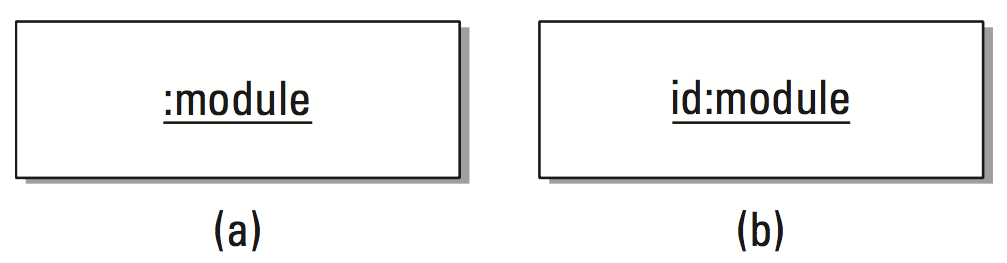
\includegraphics[width=0.7\textwidth]{img/f3-2.png}
			\caption{Instâncias e suas descrições. Fonte: \cite{Sass2010}.}
			\label{fig:instance}
		\end{figure}

		Como exemplificação, pode-se construir um somador completo de 4-bit utilizando várias instâncias da implementação do somador completo de 1-bit, exibido na Figura \ref{fig:somador_instancias}.

		\begin{figure}[h] \centering
			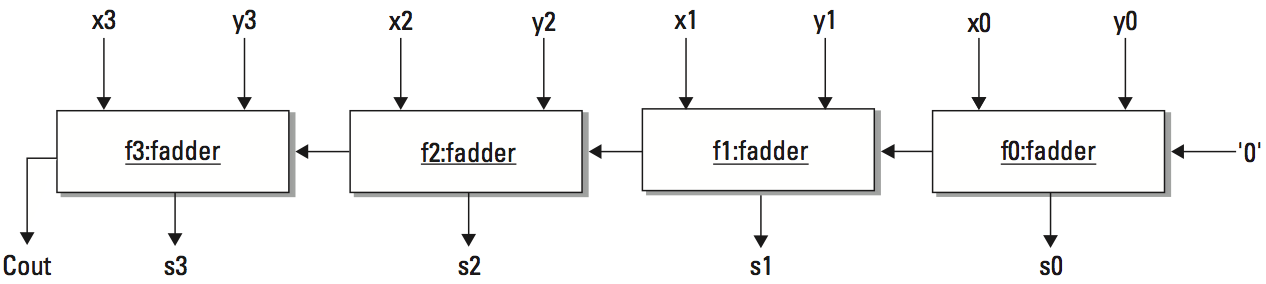
\includegraphics[width=0.98\textwidth]{img/f3-3.png}
			\caption{Somador completo 4-bit utilizando instâncias de 1-bit. Fonte: \cite{Sass2010}.}
			\label{fig:somador_instancias}
		\end{figure}
	\end{comment}

\begin{comment}
	\subsubsection{Abstração e Estado}
	\subsubsection{Coesão e Acoplamento}
\end{comment}


\subsection{Ferramenta \Profile} \label{sec:profile}

		\Profile\ é uma técnica para coletar informações do \software\ em tempo de execução. O \software\ referencial é executado com uma entrada representativa e o tempo gasto em várias partes da aplicação é mensurado. 
        %A Figura \ref{fig:f4-1} exibe um exemplo gráfico de \profile\ de \software\ em um codificador de imagem.

		Uma das técnicas do \profile\ de mensurar uma aplicação é realizar interrupções periódica no programa e amostrar o seu \textit{program counter}. Dessa forma, é possível utilizar um histograma para contar quando um programa é interrompido em um endereço particular e a partir dessa informação, calcular a fração aproximada do tempo total de execução gasto em suas partes. Distribuições GNU/Linux possuem a ferramenta \texttt{gprof} que realiza o cálculo de tais informações de \software\ \cite{Graham1982}.



\subsection{Sistemas Computacionais \Wearables}
	% Introdução histórica e geral
	Sistemas computacionais \wearables\ são sistemas que, com a possibilidade de ter um computador acoplado ao corpo, proporciona-se ao usuário um nível superior de informações contextualizadas dentro de um ambiente interativo \cite{Amorim2017}.

	\todo{intowearaable}

	Devido ao movimento de seus usuários, um computador \wearable\ é embutido em um ambiente \mobile\ e necessita-se da interação com seu ambiente ao seu redor \cite{Plessl2003}.
	Um sistema \wearable\ é composto por um conjunto de nós distribuídos e uma rede de comunicação centralizada num módulo principal, sendo possível determinar, por exemplo, a geração de eletricidade por meio de geradores \textit{piezo-electric} integrados aos sapatos, energizando uma parte do sistema \wearable\ com o caminhar do usuário \cite{Kymissis1998} ou a ação do usuário por meio de acelerômetros \cite{VanLaerhoven2002, Kern2002}.

	Com a distribuição espacial dos módulos pelo corpo, a comunicação torna-se um item importante em termos consumo de energia \cite{Kymissis1998}. A rede de comunicação é uma mistura de conexões cabeadas e sem-fios. Para dispositivos \wearables, a comunicação sem-fio é a tecnologia predominante \cite{Plessl2003}.

	A introdução desses sistemas no ambiente de pesquisa não é nova como é reportado por \cite{Sutherland1968}, \cite{Mann1996} e \cite{Mann1997}. Entretanto, a aplicação desses, depende diretamente da miniaturização dos componentes eletrônicos. Esse fenômeno é claro com o crescente espaço ganho nas indústrias e nas atividades pessoais de usuários pelos \textit{smartwatches}, \textit{fitness trackers}, óculos, equipamentos de realidade virtual e aumentada e muitos outros. Com esses novos dispositivos de propósito geral minituarizados, aumenta-se a sua atração devido à fácil disponibilidade dos dispositivos, baixo preço e ferramentas de desenvolvimento disponíveis para desenvolvimento de aplicações específicas incluindo compiladores e sistemas operacionais para tal, mas não são otimizados para uso \wearable.
	\cite{Plessl2003} cita que em \cite{Plessl2003}, muitos dos sistemas \wearables\ construídos possuíam características diferentes de componentes que prestam auxílio em tarefas pessoais de usuários, citados anteriormente.
	Por exemplo, o uso dados de teclados, canetas para entrada de dados ou um \textit{display} LCD contradiz com o paradigma de operações \textit{hands-free} e a propriedade de computação \wearable\ discreta.
	Sistemas de computação distribuídos no corpo construídos a partir desses equipamentos são altamente ineficientes devido à falta de especialização de componentes individuais de propósito específico.
	Dessa forma, a computação \wearable, seguindo esse conceitos, se define muito bem como um subconjunto de sistemas embutidos.

	% Característica de um dispositivo wearable
	\subsubsection{Característica de um \Wearable}

		A caracterização de um dispositivo \wearable\ é feita acordando às classificações pré-estabelecidas em relação à suas funcionalidades e requisitos de \hardware. O mercado possui um número considerável de dispositivos \wearables\ que são utilizados em inúmeras áreas e mesmo que cada equipamento separado tenha suas próprias características, muitas soluções em \hardware\ compartilham uma arquitetura e organização de recursos implementados interna comum.
		Esses detalhes também podem ser expandidos às características relativas a recursos de sistemas operacionais, no qual dispositivos \wearables\ podem ser classificados além de seus componentes de \hardware\ internos como suas funções de performance \cite{Delabrida2016, Amorim2017}, como representado pela Figura \ref{fig:classification}.

		\begin{figure}[h] \centering
			\vspace{-10pt}
			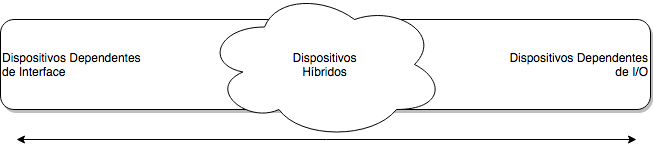
\includegraphics[width=0.45\textwidth]{img/rt-gradiente.png}
			\vspace{-10pt}
			\caption{Classificação de sistemas \wearables. De um extremo existe os dispositivos dependentes de interfaces de usuário e do outro os dependentes de entrada e saída de sinais enquanto entre eles, a gama de combinações possíveis.}
			\label{fig:classification}
		\end{figure}

		De um lado desta gama de dispositivos existem os dispositivos dependentes de interfaces de usuário que possuem alta dependência com operações interfaces gráficas, provendo respostas sobre as interações do usuário.
        Esses dispositivos focam principalmente em tarefas para renderização em \textit{displays} como por exemplo equipamentos de realidade virtual e aumentada para implementação de objetos tridimensionais.

		De outro lado existem os dispositivos dependentes de entrada e saída de sinais. Esses dispositivos atuam principalmente com o estímulo por algum dado oriundo de outro dispositivo ou do ambiente assim entregue à nuvem respeitando restrições de tempo real.
        Isso se da pela utilização de sensores acoplados ao dispositivo que podem exigir uma boa vazão de dados e pequena latência como são os monitores de atividade remota, situação na qual cria-se o ambiente perfeito para o termo conhecido por \textit{Internet of Things} (IoT).

		Entre dispositivos dependentes de interfaces de usuário e de entrada e saída de sinais existe os híbridos. São dispositivos que utilizam recursos de ambos os extremos citados.
        Dispositivos como \textit{Smartwatches} e \textit{fitness trackers} são exemplos de tais dispositivos híbridos no qual possuem restrições de equalização a prioridade dada pelo dispositivo para ambas as operações de interface e sinais.

		A separação dos conceitos computação \wearable\ e IoT ainda não estão claros segundo a bibliografia. Sistemas operacionais de propósito específico para ambientes \wearable\ são comumente focado em um único tipo de seguimento de produto como os \textit{smartwatches} sendo um meio que proporciona aos desenvolvedores um meio para sua aplicação final além de entregar um produto de alta qualidade.
        Entretanto, atualmente não existe nenhum sistema que satisfaça todos os requisitos apresentados \cite{Amorim2017}.

		Já \cite{Jozwiak2017} em seu trabalho caracteriza um sistema \wearable\ como um sistema \textit{cyber}-físico\footnote{Sendo \textit{cyber-} uma combinação dos termos `computador', `rede de computadores' ou  `realidade virtual' com um segundo termo, no caso o `físico' oriundo de circuitos.} móvel autônomo.
        São sistemas que podem ter mobilidade inerente ou poder ser transportado para outro sistema, industrial ou natural (incluindo humanos), sendo autônomos em termos de funcionalidade.
        Podem ser utilizados para aplicações de consumidores (computação móvel), extensões ou reposição de capacidades humanas, sistemas sociais (\textit{health-care} inteligente), automotivo, industrial (monitoramento) e aplicações comerciais como realidade aumentada para informações turísticas.
		Eles representam uma grande parte da heterogeneidade de sistemas embarcados, cobrindo muitos campos e tipos de aplicações que vão desde um dispositivo inteligente integrado à roupa, focado no campo de computação \textit{mobile} pessoal, até indústrias como dispositivos de segurança. % \cite{Jozwiak2017}.
        Esses dispositivos podem também trabalhar de forma colaborativa com \textit{smartphones}, redes e outros sistemas criando um sistema mais complexo.

		Segundo \cite{VanLaerhoven2002}, a distribuição de sensores se adequ à pesquisa que aumenta objetos mundanos com elementos computacionais, comumente designados por computação ubíqua, o que afirma também que computação \wearable\ também não foge do conceito uma vez que superfícies de roupas são uma plataforma de suporte ideal para uma grande quantidade de sensores (desde que sejam miniaturizados para que eles não obstruam o usuário).
		Essa restrição de tamanho geralmente significa que a própria qualidade do equipamento também está comprometida, o que leva ao conceito de muitos atuadores e sensores simples.

		Sistemas \wearables\ são uma subclasse de sistemas embutidos distribuídos e por causa disso, são sujeitos à várias restrições de \design sendo elas performance em multi-nós, gasto energético consciente e alta flexibilidade \cite{Plessl2003}:
        \begin{itemize}
        	\item \textbf{Performance de multi-nós:} Requerem um performance base fixa para tarefas que não mostram altas demandas computacionais nem restrições de tempo rigorosa.
            Sistemas \wearables\ executam rajadas de tarefas de computação intensiva que consideram restrições de tempo-real. Não realizando as tarefas, o sistema torna-se inaplicável.

			\item \textbf{Gasto energético consciente:} É essencial em sistemas na medida que ele deve-se manter ativo e funcional num certo período de tempo. O \design\ do gasto de energia conduz inúmeros desafios como gerenciamento computacional energético eficiente e energização dinâmica. Diferenciando os termos de baixo custo de energia e eficiência energético, o consumo de energia é mensurado pela divisão da dissipação energética pelo tempo mensurado.

            A eficiência energética relaciona o total de energia necessário para computar uma tarefa específica sendo o desafio a construção de um \design\ na qual possui-se alta eficiência energética para um dado conjunto de tarefas. O procedimento dinâmico de energização consiste na tarefa de associar determinada tarefa para o componente mais eficiente (energeticamente falando) disponível e forçar todos os outros não utilizados pelo sistema a serem postos em modo de economia de energia ou desligá-los quando apropriadamente.

			\item \textbf{Flexibilidade:} Quando menciona-se sobre alta flexibilidade, é considerado o fato de que o dispositivo será utilizado em situações altamente dinâmicas. Isso fica claro na necessidade na qual os requisitos de aplicação variam de acordo com as escolhas do usuário, mas também com o contexto e local utilizado. Outro é no fato de que o usuário troca de roupas constantemente e com isso os dispositivos devem ter a capacidade de serem acoplados e removidos, neste caso. Isso além de critérios como confiabilidade, disponibilidade e fatores dependentes de sua forma como volume e peso.
        \end{itemize}

		Dessa forma, pode-se estabelecer que os requisitos flexíveis em um sistema \wearable\ demanda um sistema de computação programável de propósito geral, enquanto os requisitos de alta performance e consumo de energia consciente demandam um sistema computacional especializado. Dessa forma, como meio para solução desses problemas, \cite{Plessl2003} utilizaram-se de um \hardware\ reconfigurável para incoporar ao sistema. O trabalho exibe um sistema \wearables\ compreendendo de um processador de até médio porte em termos de processamento e módulos reconfiguráveis.
		A utilização de \hardware\ reconfigurável nos permite alcançar alto processamento com maior eficiência energética em relação à processadores para tarefas de computação intensiva em tempo real.
